%%%%%%%%%%%%%%%%%%%%%%%%%%%%%%%%%%%%%%%%%%%%%%%%%%%%%%%%%%%%%%%%%%% 
%                                                                 %
%                            CHAPTER                              %
%                                                                 %
%%%%%%%%%%%%%%%%%%%%%%%%%%%%%%%%%%%%%%%%%%%%%%%%%%%%%%%%%%%%%%%%%%% 

\chapter{Conclusion and future research}
\label{ch:Conclusions}

\paragraph{Problem definition} 

The best way to analyse DNA in detail is to sequence it. This will determine which bases and in which order they are occuring in the DNA. However, the most commonly used technology of DNA sequencing machines limit us to reads of 75-300 bases long. If we want to make assumptions about the whole genome, we will need to input a lot of these reads. 

Typically, each read is compared with the whole genome in a local alignment, for example with the Smith-Waterman algorithm. As an output, we would get the position in the human genome and an alignment with its score (how well the sequence fits in that spot). This practice is commonly referred to as \emph{Mapping to a reference genome}.

Sequencing machines produce millions of the reads in a sequencing experiment. Since every read from DNA sequencing machines are 75 to 300 bases long, and the whole human genome is approximately 3 billion bases, this mapping is computationally a very intensive task. If we analyze the S-W algorithm (as we have done in Subsection~\ref{expl:SWanalyse}), we can see that the value of each cell in the matrix is only dependent on the left-upmost 3 cells. Therefore, it leads us to believe that this algorithm can be accelerated on hardware solutions such as an FPGA (as discussed in Chapter~\ref{ch:Platforms}) since the S-W algorithm is heavily parallelizable.

In most clinical applications where mapping to a human reference genome is used, the number of reads to be compared with the genome is in the millions, which further increases the demand to speedup the process of mapping the reads in the genome, to decrease the time-to-result.

The idea of this thesis was to implement the Smith-Waterman alignment algorithm on an MPSoC, which contains both programmable FPGA hardware and an ARM processor in 1 chip. As a target board, the ZCU 104 evaluation kit was chosen.

\paragraph{Proposed solution and implementation}

As a starting point, a software implementation was implemented on the ARM processor. After running the software implementation overnight with the unmapped sequences from the coronavirus as a sample set, we obtained a dataset of mapped reads. The reads were also mapped by using the Galaxy online tool~\cite{} and both were imported into the IGV analyzing software for visualisation and comparison, which can be seen in figure~\ref{fig:IGVcomparisonConcl}

\begin{figure}[H]
	\centering
	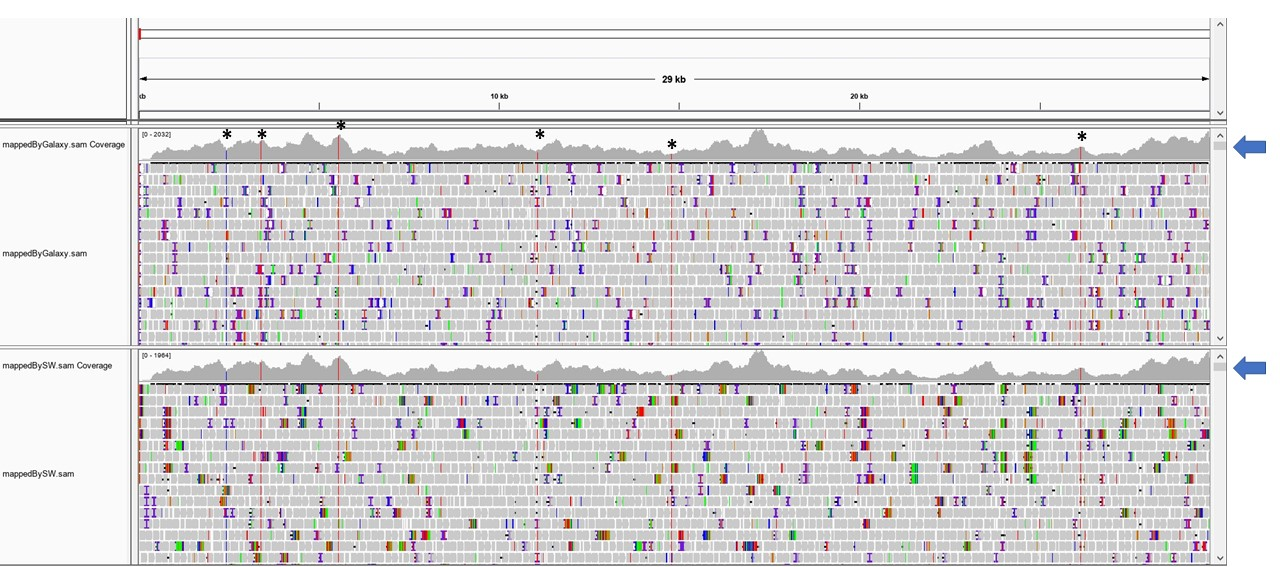
\includegraphics[width=\textwidth]{softwareResults/comparison.jpg}
	\caption{A comparison of the data obtained by Galaxy (top) and the data obtained by the implementation discussed in this chapter (bottom)}
	\label{fig:IGVcomparisonConcl}
\end{figure}

It can be observed that the implementation is working correctly since the reading depth graphs are approximately the same (indicated by an arrow). If we look closely to figure~\ref{fig:IGVcomparisonConcl}, some small differences between the exact reads are visible. This will probably be because both the algorithm and the parameters were a bit different. However, the important part is that the reading depths are the same, as well as the consistently mutated bases marked in the genome (indicated by an asterisk).

\paragraph{Hardware speedup}

After implementing the matrix fillIn in the FPGA hardware, we can examine execution time (using the built-in latency analyzers in SDSoC). The estimated achieved speedup was 4.41x. This means the hardware variant of the implementation runs 4.41 times faster than the software variant.

\begin{figure}[H]
	\centering
	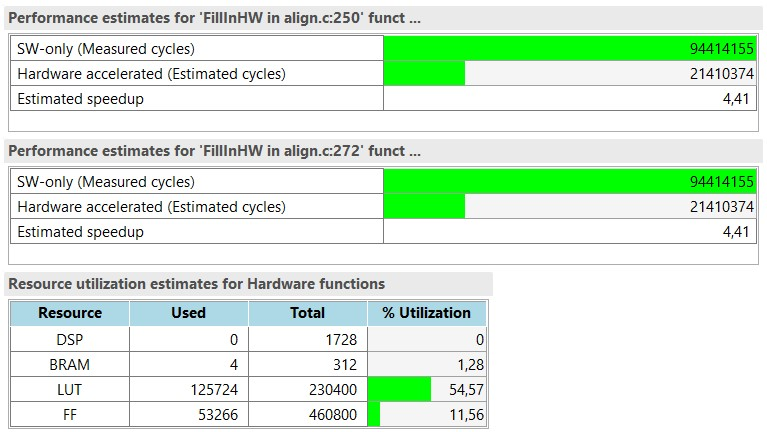
\includegraphics[width=0.8\textwidth]{speedup/speedup.jpg}
	\caption{The latency analyzer in SDSoC. We can see the number of clock cycles spent in the software and the hardware variant of the implementation, as well as the speedup. The speedup is calculated 2 times, since we run the fillIn function twice, once for the forward and once for the reverse sequence. The resource utilization of the FPGA hardware is also visible in this picture}
	\label{fig:speedupConcl}
\end{figure}





\paragraph{Future work - recommendations for improving the current implementation}

the following optimizations could improve the proposed implementation:

\begin{itemize}
	\item Treat the alignement gap opening and extension separately. In the current implementation, the gap penalty is treated linearly. However, the S-W algorithm could be refined to include an affine gap penalty. More info on the gap penalty can be found at Subsection~\ref{expl:SWanalyse}.
	\item In a sequence, a base position may be suddenly marked with an 'N' character, which represents a base that was unidentified in the primary processing. In this thesis, it was decided to cut the sequence short at the moment an 'N' character is registered. However, a possible improvement might be to keep these unidentified bases in the alignment as a "generic" base and in this way improve the accuracy of the alignment. More info on the current implementation can be found at Subsection~\ref{codeStructure}.
	\item Make some types more memory efficient, such as the BASE and the SEQ\_INDEX type. Firstly, the BASE type only has 4 possible values (the 4 nucleotide bases). However, it is defined as 1 byte in the current implementation, since it is the smallest type that C supports. However, storing a base in 1 byte is memory inefficient. Improvements could be made by defining an own type, by stacking 4 bases in 1 byte. Secondly, the SEQ\_INDEX type is stored as 2 bytes in the current implementation, even though it only contains values up to 300, which makes it memory inefficient. This could also be improved.
	\item If this implementation would be used in practice, there would be a need to find an easier way to on and offload data to board. Currently,  this is accomplished by changing out the SD card, which could easily be improved using FTP since an Ethernet stack is, which are already implemented by the operating system. The speed the data would be transferred at, is not important since we can assume the time it takes to map the sequence takes far longer. 
\end{itemize}

\paragraph{Future work - recommendations for re-evaluating the alignment method}

In the field of alignment algorithms, a few alternatives exist to S-W since it takes a lot of computing power. In most cases, these algorithms will use a transformation or a lookup table to determine possible candidate locations, where a small regional S-W will be performed on a part of the genome. For example, The BFAST algorithm uses a hash table where candidate locations are stored for every sequence~\cite{fpgaImpl}. As a second example, in the Bowtie application, the candidate locations are determined using the Burrows-Wheeler Transform.

As future work, one of these more sophisticated algorithms can be selected. Some candidate locations can then be determined in a way defined by the algorithm. These candidate locations can then be mapped using the implementation of this thesis.